\section{Reconhecimento de marcadores}
\label{sec:reconhecimentoMarcadores}	
	
		O processo de reconhecimento dos marcadores é dividido em etapas bem definidas. No entanto, estas
		podem ser implementadas de formas diferentes levando-se em consideração a aplicação utilizada.
		Esse processo tem o objetivo de identificar objetos com formatos pré-definidos e que possuam
		códigos de identificação compatíveis com a aplicação. A partir desse
		reconhecimento é possível estabelecer o posicionamento dos objetos em relação ao dispositivo
		responsável pela captura da imagens e apresentar o objeto virtual correspondente sobreposto ao
		marcador reconhecido. As etapas envolvidas nesse processo são apresentadas na
		figura~\ref{fig:pipelineAR} e dividas da seguinte maneira:
		
		\begin{figure}[htb]
			\centering 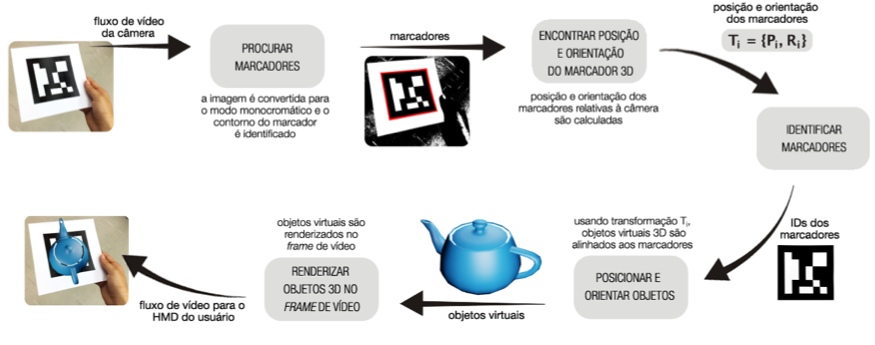
\includegraphics[scale=.55]{figuras/cap2/pipelineAR.png}
			\caption{\textit{Etapas do processo de reconhecimento de marcadores na Realidade
			Aumentada~\cite{fpga}.}}
			\label{fig:pipelineAR} 
		\end{figure}
		
		\begin{enumerate}
		  \item \textbf{Procurar marcadores}
		  
				O fluxo de vídeo obtido por uma câmera é entrada da etapa inicial do processo de
				reconhecimento. Ele é lido e encaminhado para o sistema de rastreamento. Neste, aplica-se uma
				operação de detecção de bordas como uma etapa inicial. Faz-se um reconhecimento de
				cada~\textit{pixel} dentro de um segmento para que seja feita um agrupamento de~\textit{pixels},
				a fim de se achar uma forma quadrangular e reconhecer a figura como um possível marcador. Esse
				método acaba sendo mais eficaz quando comparado com o método de derivar o marcador a partir de
				uma intensidade de luminosidade de escala de cinza, devido o seu reconhecimento em ambientes de
				pouca luminosidade e problemas relacionados com oclusão (parte da visualização do marcador é
				obstruída por um outro objeto)~\cite{artag}.
				
			\item \textbf{Encontrar posição e orientação do marcador 3D}
			
				Nesta etapa o marcador já foi encontrado na imagem. Para obter uma estimativa da posição do
				marcador é necessário obter quatro pontos não lineares e identificáveis na imagem. Estes pontos
				devem aproximar a um formato correspondente a um quadrado. Na situação de identificação das
				posições baseados na utilização de várias câmeras, envolve a localização do mesmo recurso em
				duas imagens obtidas por câmeras diferentes. Isso possibilitaria estimar a posição geométrica
				tridimensional de um recurso. Neste caso para estimar a localização de tal recurso necessitaria
				combinar as informações de três pontos não lineares. Alguns problemas podem ser detectados, como
				por exemplo, a distorção de perspectiva ocorrendo quando o plano da tela não é o mesmo plano do
				marcador~\cite{kler}.
				
			\item \textbf{Identificar marcadores}
			
				É nesta etapa que acontecem mais particularidades para o reconhecimento dos marcadores
				observadas em diferentes aplicações. Na aplicação ARTag, o conteúdo extraído do interior do
				marcador é preenchido com uma matriz quadrada 6 x 6 com células de cores preto e branco, aos
				quais representarão valores binários de 0's e 1's. Essa matriz retornará uma sequência de
				36~\textit{bits}, sendo analisada de quatro formas distintas por causa das quatro rotações
				possíveis para o marcador.
				
				O código identificador do marcador é constituído por 10 \textit{bits}, sendo codificado a
				partir da sequência dos 36~\textit{bits} obtidos e deixando os 26~\textit{bits} restantes para a
				detecção e correção de erros, bem como a unicidade em torno das quatro possibilidades de rotação
				do marcador~\cite{hirzer}. São utilizados os métodos~\textit{CRC (Cyclical Redundancy Check)}
				e~\textit{Forward Error Correction} para detecção do marcador e extração do seu número
				identificador correspondente, adicionando o conceito dos operadores lógicos XOR para codificação
				e decodificação. A correção e reparo dos erros, desalinhamento de fronteira, oclusão, dentro
				outros, fica sobre a responsabilidade do~\textit{FEC (Forward Error Correction)}. Outros
				métodos, baseados em probabilidades, também são aplicados para garantir o reconhecimento correto
				do identificador do marcador em relação aos demais marcadores.
				
				A figura \ref{fig:artagDecoding} exemplifica os passos necessários utilizado pelo ARTag para
				obter o código de identificação do marcador a partir do marcador reconhecido nas etapas anteriores 
				do~\textit{pipeline}.
				
				\begin{figure}[h]
					\centering 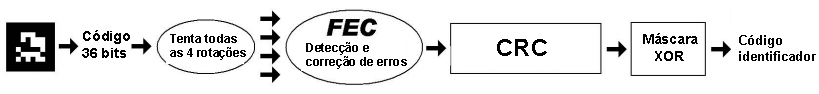
\includegraphics[scale=.55]{figuras/cap2/artag_decoding.png}
					\caption{\textit{Obtenção do código identificador do marcador. Adaptado de~\cite{artag}.}}
					\label{fig:artagDecoding} 
				\end{figure}
				
				De forma análoga, o ARToolkit extrai o conteúdo do interior do marcador e gera uma matriz
				quadrada. No entanto, as dimensões dessa matriz são de 16 x 16 ou 32 x 32. Os valores obtidos
				por essa matriz geram um vetor característico que é comparado com uma biblioteca de vetores
				característicos conhecidos e geram como resultado um fator de confiança para dizer se o
				marcador foi reconhecido.
				
			\item \textbf{Posicionar e orientar objetos}
			
				Nesta etapa, os objetos virtuais 3D são identificados e associados de acordo com o marcador
				identificado na etapa anterior. Os mesmos são alinhados ao marcador pelo posicionamento obtido na
				etapa 2.
			
			\item \textbf{Renderizar objetos 3D no ~\textit{frame} de vídeo}
			
				Por fim é gerado o \textit{frame} de vídeo, contendo o marcador e seu respectivo objeto virtual
				3D. Após ser renderizado, o mesmo é repassado para o objeto de visualização de vídeo, podendo ser um
				monitor,~\textit{HMD} ou \textit{smartphone}.
				
		\end{enumerate}
	
		A quantidade de marcadores, aos quais podem ser geradas com uma boa qualidade de reconhecimento
		varia para cada tipo de aplicação. Essa qualidade de reconhecimento refere-se a símbolos no
		interior dos marcadores aos quais são facilmente distinguíveis pelas aplicações. Isso mostra 
		que a quantidade de \textit{bits} obtidos a partir da matriz gerada pelo interior do marcador,
		pode-se construir diversos símbolos. No entanto, pela isomorfia dos marcadores (rotação do marcador 
		em 0, 90, 180 e 270 graus) muitos símbolos acabam sendo descartados por se tratar do mesmo marcador. 
		No ARTag e no ARToolkitPlus, esses números são bastantes diferentes.
		Enquanto que no primeiro, 2002 marcadores são reconhecidos facilmente, no segundo esse número cai
		para 512. Porem, muitos outros símbolos podem ser gerados, mas sem muita garantia de uma boa
		qualidade em seu reconhecimento. Não foi possível obter as mesmas informações a respeito da
		quantidade de marcadores que são reconhecidos pelo ARToolkit.
		
	
